\documentclass[a4paper,12pt,twoside]{report}

\usepackage[left=3cm,right=3cm,top=3cm,bottom=3cm]{geometry} %Margins
\usepackage{pdfpages}
\usepackage{hyperref}
\usepackage{listings}
\usepackage{xcolor}
\usepackage{setspace}
\usepackage{tocloft}
\usepackage{amsmath}
\usepackage{chngcntr }
\usepackage[toc,page]{appendix}
\usepackage[T1]{fontenc}
\usepackage[nottoc]{tocbibind}
\usepackage[compact]{titlesec}
\usepackage{float}

\usepackage[utf8]{inputenc}
\usepackage{amsmath, amssymb, latexsym}
\usepackage{sidecap}
%---tikz---
\usepackage{tikz}
\usetikzlibrary{decorations.pathreplacing}
\usetikzlibrary{fadings}

\titlespacing{\section}{0pt}{1ex}{0ex}
\titlespacing{\subsection}{0pt}{1ex}{0ex}
\titlespacing{\subsubsection}{0pt}{1ex}{0ex}

\counterwithout{figure}{chapter}
\counterwithout{table}{chapter}

\include{thesis.preamble}

\begin{document}

\newgeometry{left=2cm,right=2cm} %Only for the title new margins

%Title parameters
\title{%
  Uncovering underlying musical content in the temporal domain \\
  \small Leveraging deep learning, inductive bias, and aural skills to learn embedding spaces for downstream MIR tasks}
  
\author{\href{oriol.colome.font@epidemicsound.com}{Oriol Colomé Font}}
\submitdate{July 2023}
\supervisor{Carlos Lordelo and Carl Thomé}
\cosupervisor{Frederic Font}

\hypersetup{
pdftitle={Your PDF title},
pdfsubject={Your PDF subject},
pdfauthor={Oriol Colomé Font},
pdfkeywords={Music; 
Music Theory; 
Music Information Retrieval; 
Music Structure Analysis; 
Machine Learning; 
Neural Networks; 
Deep Learning}
}

\maketitle

\restoregeometry

\preface
\cleardoublepage 

%\addcontentsline{toc}{chapter}{Acknowledgement}
\begin{dedication}
\pagenumbering{gobble}% Remove page numbers (and reset to 1)
I dedicate this master's thesis to my closest family and friends, who have supported and inspired me throughout this journey. Their unwavering love and encouragement have motivated me to pursue my academic goals, and their belief in me has never faltered. I am grateful for their patience, understanding, and sacrifices as I pursued my studies. 

Their presence in my life has made this journey meaningful, and this thesis is a tribute to their support. 

\newpage

\end{dedication}


%\addcontentsline{toc}{chapter}{Acknowledgement}

\begin{acknowledgement}
\pagenumbering{gobble}% Remove page numbers (and reset to 1)

I want to extend my deepest gratitude to...

\begin{itemize}
\item Carlos Lordelo and Carl Thomé for their invaluable guidance and support throughout my thesis. Their MIR, ML, and DSP expertise has been instrumental in shaping my research and driving it toward success. I am truly grateful for their unwavering support and encouragement, which helped me surmount any difficulties I encountered during this journey. Their time, effort, and dedication in mentoring me have not gone unnoticed. They inspire me with their commitment to their students, and I feel honored to have had the opportunity to work with them.

Words fall short of my profound gratitude for their consistent, knowledgeable, and steadfast support. I am beyond grateful that their dedication has left an indelible mark on my academic journey.

\vspace*{3mm}
\item Cody Hesse and Sebastian Löf
\vspace*{3mm}
\item The Music Technology Group (MTG)
\vspace*{3mm}
\item My colleague at My Sheet Music Transcriptions, Oriol López, for his exceptional support and flexibility throughout my thesis. His understanding and willingness to accommodate my academic commitments effectively allowed me to balance my work and research responsibilities.
\vspace*{3mm}
Thank you all for being excellent advisors and playing a crucial role in completing my thesis. I sincerely appreciate everything you have done for me and will always cherish the knowledge and experience I have gained under your guidance.
\vspace*{3mm}
\end{itemize}

\newpage
\end{acknowledgement}
%\addcontentsline{toc}{chapter}{Acknowledgement}
\begin{preface}
\pagenumbering{gobble}% Remove page numbers (and reset to 1)

Music and science have always been my two greatest passions. When the opportunity to work at Epidemic Sound presented itself, it was as if the universe had conspired to bring my interests together, offering me the chance to explore the fascinating field of MIR from an industrial perspective. With the support and encouragement of my loved ones, I took a leap of faith and moved to Stockholm to embark on this exciting journey.

This work aims to help untangle the complexities of music and offer a more musically-driven perspective to MIR. I aim to contribute to a deeper understanding of the intricate relationships within musical data by bridging the gap between music theory and computational analysis.

I am deeply grateful to the Epidemic Sound team for their guidance, expertise, and camaraderie throughout this project. I would also like to extend my heartfelt appreciation to my family for their unwavering support and belief in my abilities.

My motivation for writing this piece stems from a desire to grow as a musician, programmer, professional, and individual. I believe that by delving into the world of MIR, I can expand my horizons while making a meaningful contribution to the field.

This work is intended for any curious human being, regardless of their background in music or computer science. I hope it will inspire others to explore the captivating intersection of these two disciplines.

The scope of this work encompasses a range of MIR tasks and methodologies, as well as discussions on the challenges and opportunities that arise within the field. Despite the ambitious nature of this project, I acknowledge that time and my academic background limitations may have constrained the depth of my analysis. Nevertheless, I hope this work will serve as a starting point for further exploration and inspire new ideas in the realm of MIR.

\newpage
\end{preface}
%\addcontentsline{toc}{chapter}{Abstract}

\begin{abstract}
\pagenumbering{gobble}

This thesis posits the existence of high-level musical concepts invariant to sonic qualities that evolve and unfolds through time. This idea parallels the nature of the symbolic domain, which maintains its essence despite being interpreted through diverse performances using various instruments and styles.

This research, conducted in collaboration with Epidemic Sound AB and the Music Technology Group (MTG) at Universitat Pompeu Fabra (UPF), employs self-supervised contrastive learning of musical representation to uncover the fundamental structure of Western tonal music. 

Embracing a subtle novel approach, this process is facilitated by using deep neural networks with a triplet loss, somewhat mimicking human aural skills in interpreting music to discern abstract and semantic musical elements, irrespective of the sonic qualities. The study replaces traditional acoustical features with deep audio embeddings to compute high-level, sound-agnostic, and content-sensitive music identification.

Results XXXXXX TBC

The preliminary results suggest that our approach to learning musically-informed embeddings holds significant potential for nearly all MIR downstream tasks. Music-motivated embeddings represent a promising technique, adaptable potentially to other tasks hindered by data scarcity. This method could significantly influence advancements in intelligent music recommendation systems and the efficient enforcement of intellectual property rights. 

\bigskip
Keywords: Music Information Retrieval; Music Structure Analysis; Deep Audio Embeddings, Aural Skills

\newpage
\end{abstract}

\body

%Introduction of the project
\normallinespacing

\chapter{Introduction}

Music, an essential component of human culture, history, and society, has existed since ancient times. It reflects the changes in our cultures, traditions, and beliefs as it evolves. Studying music, however, has always been a challenging and complex task due to its subjective nature and the sheer variety of musical styles, genres, and cultures that exist worldwide.

For millennia, people have sought to understand the underlying structure of music. Music has captivated and intrigued us from the ancient Greeks to the present day. This rich music theory and analysis history form a valuable foundation for guiding and evaluating Music Information Retrieval (MIR) algorithms and models.

Music Information Retrieval (MIR) has emerged over the last few decades as an interdisciplinary field that combines engineering, musicology, and neuroscience. It aims to develop algorithms and techniques for automatically analyzing, classifying, and retrieving musical information, primarily from audio signals. While MIR research has traditionally focused on technical aspects such as Digital Signal Processing (DSP) and pattern recognition, it may have overlooked other relevant domains, including perception, cognition, music theory, aural skills, and musicology, along with their subfields.

\subsubsection{Bridging the gap}

Music similarity is a critical factor in query-by-example retrieval systems. However, similarity calculation and definition can differ depending on user needs and retrieval scenarios. While acoustic properties like voice, genre, melody, tempo, instrumentation, and rhythm contribute to similarity, personal preferences, and cultural context also play a significant role. For instance, a user may avoid a particular artist's music despite its similarity to their favorite artists due to the album cover. Moreover, the user's context, such as driving or running, can also influence their preference and perception of similarity. 

Metadata is the traditional approach to electronic music searches, but it can be impractical and unintuitive for users who are unfamiliar with most tracks. Retrieval systems often overlook the cultural, personal, and musical aspects of music information needs, rendering them less useful for non-expert users. Many people search for music based on emotions or usage context rather than bibliographic information.
\section{Motivation}
As a music lover, professional musician, and connoisseur, I am interested in gaining a deeper understanding of the fundamental building of musical composition, the various techniques used to create musical works, and capturing underlying relationships among them. I am deeply interested in learning how to retrieve useful embedded information within the music. 

\subsection{Beyond Digital Signal Processing (DSP)}

We argue that MIR research needs to incorporate a more balanced approach that considers the interdisciplinary nature of music and the importance of other domains beyond DSP.

Let's pick a core MIR task as a sample to display such complexity: Music Structure Analysis (MSA), an interdisciplinary field that aims to understand the structure of music\cite{Nieto2020Audio-BasedApplications}. However, due to subjectivity, ambiguity, and data scarcity, audio-based MSA faces challenges like boundary placement ambiguity and similarity quantification \cite{NietoPerceptualMusic}. The main principles of MSA were initially defined as homogeneity, novelty, and repetition, with the addition of regularity.

The checkerboard kernel technique is a simple and effective method for Music Structure Analysis (MSA) based on the homogeneity principle. The kernel, with a checkerboard-like structure, is convolved over the main diagonal of a Self-Similarity Matrix (SSM) such as $S_{ij}$ is the similarity between time frames $i$ and $j$, $\vec{x}_i$ is the vector representation of time frame $i$, and $\left| \vec{x}_i \right|$ is the Euclidean norm of vector $\vec{x}_i$. The dot product of two vectors $\vec{x}_i$ and $\vec{x}_j$ is denoted by $\vec{x}_i \cdot \vec{x}_j$.

\begin{equation}
\label{eq:segment_similarity}
S_{ij} = \frac{\vec{x}_i \cdot \vec{x}_j}{\left\| \vec{x}_i \right\| \left\| \vec{x}_j \right\|}
\end{equation}

This yields a novelty curve that highlights sudden changes in the selected musical features (some examples would be chroma, MFCCs, beat-synchronous features, onset and offset detection, and harmonic and percussive separation) from which to extract the segment boundaries.

\begin{equation}
\label{eq:novelty_curve}
n_i = \frac{\sum\limits_{j=1}^{N} S_{ij} - N\cdot S_{ii}}{\sqrt{\sum\limits_{j=1}^{N} (S_{ij} - S_{ii})^2}}
\end{equation}

Where $N$ is the number of time frames, $S_{ij}$ is the similarity between time frames $i$ and $j$, $S_{ii}$ is the similarity between time frame $i$ and itself, and $n_i$ is the novelty value for time frame $i$.

The numerator of the expression \ref{eq:novelty_curve} represents the sum of similarities between time frame $i$ and all other time frames minus the average similarity across all time frames. The denominator of the expression is the standard deviation of the similarities, which is used to normalize the values to ensure that the novelty values are between -1 and 1.


Mathematical operations are used on predefined principles such as homogeneity and repetition to analyze a musical structure. It analyzes features extracted from a musical signal and identifies peaks in a novelty curve to extract segment boundaries. In contrast, human aural skills rely on the perception and interpretation of music by human listeners based on cultural and academic background. They can capture subtle nuances of musical structure, but those still are subjective and can vary across listeners.

Combining technical tasks, aural skills, and music perception is challenging due to the complexity and subjectivity of musical perception, discrepancies between the features extracted by DSP techniques and the features perceived by humans, and the variability of musical signals and individual differences in musical perception. DSP techniques may not always reflect how humans perceive music and may not capture the subtle variations in timing or harmonic relationships critical to musical perception. Variability in musical signals due to instrumentation, genre, and performance style further complicates the development of DSP techniques that can be generalized to different musical contexts.

\section{About aural skills and high-level perceptual}

%%%%%%%%%%%%%%%%%%

\begin{figure}[h]
\includegraphics[clip,width=\columnwidth]{figures/schenkerian analysis/SchubertOp4no3.png}% 
\caption{Small excerpt of \textit{Wandrers Nachtlied, Op. 4, D. 224} by Franz Schubert. We can see the passage's original score, the schenkerian unfolding of the melody, the chord degrees, and the tonal function.}
\label{fig:Wandrers Nachtlied, Op. 4, D. 224}
\end{figure}

%%%%%%%%%%%%%%%%%%%%%%%%%%%%%%%%%%%%%%%%%%%%

I have consistently been inspired by researchers who strive to uncover musical ground truth within the existing tonal paradigm, such as Heinrich Schenker\cite{}, or by challenging it, as exemplified by George Russell\cite{LydianRussell}. Both approaches aim to identify abstract concepts that reinforce or disrupt the tonal foundation. Their ultimate goal is to advance the tonal landscape, providing musicians with a dependable playground for growth and development.

Schenkerian Analysis:
Schenkerian Analysis, developed by Austrian music theorist Heinrich Schenker, analyzes tonal music focusing on its underlying structure. It seeks to reveal the hierarchical relationships between pitches, based on the premise that all tonal music has a fundamental structure known as the "Ursatz" or "basic shape." The Ursatz consists of a stepwise descending line (Urlinie) supported by a bass arpeggiation (Bassbrechung). Schenkerian Analysis reduces a musical composition to its essential elements, enabling the analyst to observe how the work's various layers contribute to the overall structure. It is worth mentioning that such analysis is done in the symbolic domain.

Schenkerian analysis is a method of analyzing tonal music, focusing on hierarchical relationships between musical elements. The theory is based on the ideas of Heinrich Schenker, who sought to show that free composition was an elaboration of strict composition, particularly two-voice counterpoint. Schenker's theory includes several key concepts:

Prolongational levels: Hierarchically organized levels of elaboration, with each level representing a new freedom with respect to the rules of strict composition.
Harmony: The basic component is the Stufe (scale degree), and Schenker's theory is monotonal, meaning that the work as a whole projects a single key.
Counterpoint and voice-leading: Schenker emphasizes the importance of two-voice counterpoint and melodic fluency (stepwise motion) in both strict and free composition.
Ursatz (fundamental structure): The underlying structure from which a work originates, consisting of a fundamental line (Urlinie) and bass arpeggiation (Bassbrechung).
Schenkerian analysis is about showing how each work elaborates the background structure in a unique way, determining its identity and meaning. While the theory has been criticized for reducing all tonal works to a few background structures, Schenker argues that the focus is on individual elaboration.

George Russell's Lydian Chromatic Concept:
George Russell's Lydian Chromatic Concept of Tonal Organization is an innovative approach to understanding and organizing musical relationships. Introduced in the 1950s, the theory asserts that the Lydian mode, rather than the traditional major scale, is the accurate parent scale in Western music. The Lydian scale is characterized by a raised fourth degree, giving it a brighter and more consonant sound. Russell's concept revolves around "chord modes," derived from a chord's parent Lydian scale. This system allows for greater harmonic flexibility and a broader range of tonal colors, influencing the development of jazz and contemporary music.
\section{Objectives}

Can deep audio embeddings be learned from reordering, scrambling, and augmenting via audio effects sequences of musical information to improve unsupervised music boundary detection?

This study explores the high-level tonal structure of music by leveraging self-supervised deep neural networks, inductive bias, and aural skills to learn and analyze music embeddings that can be applied to subsequent MIR tasks, with a particular focus on music boundary detection.

Our research aims to develop and learn a unified numerical understanding (or embedding \footnote{A learned representation or embedding is a numerical output - usually a fixed-size vector - produced by a machine-learning model. Good representations should be versatile across various tasks and require limited supervision \cite{Turian2022HEAR:Representations}.}) for a piece of music that integrates the high-level relationships between musical elements as they unfold over time.

The research will employ MIR computational methodologies and musicological perspectives to explore musical compositions across various styles and genres.

This approach replicates human auditory capabilities by understanding and identifying abstract and semantic musical elements independent of their sonic qualities.
\section{Assumptions}

This thesis posits that high-level musical concepts manifest over time and remain invariant to specific attributes such as tonal quality, tempo, key, orchestration, signal noise, etc. This is akin to a sheet music composition performed in myriad ways using diverse instruments and styles while preserving its essence.

Abstract high-level features, such as melody, harmony, rhythm, tempo, form, and expression, can be identified irrespective of waveform or production style. This approach offers objective and comprehensive insight into a piece's musical content and meaning, analogous to how analyzing sheet music unveils a composition's underlying structure and intent.

Although a waveform might have limited sheet music representations that accurately encapsulate its musical components, a single sheet music composition can be performed infinitely using various instruments, voices, tempos, and interpretations. The distinct tonal quality of a waveform is significantly influenced by the specific instrument timbre or production technology employed in its creation, complicating the transcription of its sonic properties into precise sheet music notation.

Moreover, this distinct tonal quality is represented by high-level natural language concepts embedded within a rich cultural and sociological tradition.


\begin{figure}
    \centering
    \scalebox{0.9}{
    \includegraphics[width=\textwidth]{figures/images/Mahler 9 Giant Steps score.png}
        }
    \caption[Mahler's 9th Symphony, 2nd movement]{\small{A small excerpt from Mahler's 9th Symphony, 2nd movement: The melodic and harmonic contour propels through non-diatonic major thirds.}}
    \label{fig:mahler}
\end{figure}

\begin{figure}
    \centering
    \scalebox{0.9}{
    \includegraphics[width=\textwidth]{figures/images/giant steps score.png}
        }
    \caption[Giant Steps]{\small{John Coltrane's Giant Steps head: A testament to harmonic exploration, featuring rapid chord changes in non-diatonic major thirds.}}
    \label{fig:giant_steps}
\end{figure}

\begin{figure}
    \centering
    \scalebox{0.9}{
    \includegraphics[width=\textwidth]{figures/images/train interlude score.png}
        }
    \caption[Last Train Home]{\small{Pat Metheny's Last Train Home interlude.}}
    \label{fig:last_train}
\end{figure}

\section{Structure of the Report}

In this report, we have organized the information into several sections and sub-sections to provide a clear and comprehensive overview of the topic. The structure of the report is as follows:

\begin{itemize}
\item Chapter 1
  \begin{itemize}
  \item Purpose
  \item Methodology
  \item Scope
  \end{itemize}
\item Chapter 2
  \begin{itemize}
  \item Section 1
  \item Section 2
  \item Section 3
  \end{itemize}
\item Chapter 3
  \begin{itemize}
  \item Section 1
  \item Section 2
  \item Section 3
  \end{itemize}
\item Chapter 4
  \begin{itemize}
  \item Summary
  \item Recommendations
  \end{itemize}
\item References
  \begin{itemize}
  \item Sources Cited
  \end{itemize}
\end{itemize}

\newpage



%Task definition
%%\input{task definition}
%Methods
\chapter{Methods}

We propose the use of a triple siamese network to train a model for music similarity retrieval. Specifically, we aim to minimize the loss function between the anchor, positive, and negative samples by using online triplet mining.

The positive samples are created by transforming and augmenting the original samples while preserving their perceptual underlying musical language. This is achieved by using techniques such as time-stretching, pitch-shifting, and adding noise to the samples. By doing so, we aim to enhance the diversity of the positive samples and improve the model's ability to retrieve similar-sounding samples that share the same underlying musical language.

On the other hand, the negative samples are created by shuffling and scrambling the original samples while maintaining their production texture. This is achieved by using techniques such as random segment selection, time-domain filtering, and frequency-domain masking. The goal is to maintain the production texture of the samples while disrupting their underlying composition.

By using the proposed triple siamese network and online triplet mining, we aim to train a model that can effectively distinguish between similar and dissimilar samples while taking into account both their underlying composition and production texture.

\section{Materials}

\section{Convolutional Neural Network (CNN)}

A Convolutional Neural Network (CNN), is a deep-learning neural network. The architecture of a CNN is composed of several layers, including:

\begin{itemize}

\item Convolutional layers: These layers apply a convolution operation to the input data, effectively learning local patterns and features in the image. The raw audio data is typically transformed into a spectrogram or a Mel-spectrogram representation, which can be considered an image-like 2D representation of the audio data. The convolutional layers are designed to learn local patterns and features in the audio data
\vspace*{3mm}

\item Pooling layers: These layers downsample the data, reducing the spatial dimensions of the input while retaining important information. They can also be used to downsample the data and reduce the temporal dimensions of the input while retaining important information. 
\vspace*{3mm}

\item Fully connected layers: These layers connect every neuron in one layer to every neuron in another layer, allowing the network to learn non-linear combinations of the features learned in the previous layers.
\vspace*{3mm}

\item Output layer: The output layer produces the final predictions of the network.
\end{itemize}

Compared to a traditional neural network, CNNs are more computationally efficient and have less number of parameters to train. This makes them more feasible for large-scale datasets and real-world problems.

On top of that, one of the main advantages of using CNNs for audio analysis is that they can automatically and adaptively learn temporal hierarchies of features from audio data, which traditional audio processing methods may not be able to do effectively. 

\subsection{Neural Network (NN)}

%Single
\begin{SCfigure}[2\sidecaptionrelwidth][h]
	\centering
	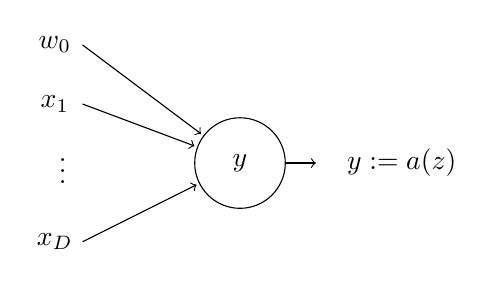
\begin{tikzpicture}[shorten >=1pt,->]
		\tikzstyle{unit}=[draw,shape=circle,minimum size=1.15cm]
 
		\node[unit](p) at (2,1){$y$};
		\node(dots) at (-0.25,1){\vdots};
 
		\draw (0,2.5) node[xshift=-10]{$w_0$} -- (p);
		\draw (0,1.75) node[xshift=-10]{$x_1$} --(p);
		\draw (0,0) node[xshift=-10]{$x_D$} -- (p);
		\draw (p) -- (3,1) node[xshift=30]{$y := a(z)$};
	\end{tikzpicture}
	\caption[Single processing units and its components.]{\small{Single processing unit and its components. The activation function is denoted by $a$ and applied to the actual input $z$ of the unit to form its output $y = a(z)$. $x_1, \ldots, x_D$ represent input from other units within the network; $w_0$ is called bias and represents an external input to the unit. The propagation rule maps all inputs onto the actual input $z$.}}
	\label{fig:processing-unit}
\end{SCfigure}
%NN
\input{Figures/Figures CNN/Network_graph}

%Backpropagation
\begin{figure}[ht]
	\centering
	% NEURAL NETWORK with coefficients, shifted
\begin{tikzpicture}[x=2.2cm,y=1.4cm]
  \message{^^JNeural network, shifted}
  \readlist\Nnod{4,5,5,5,3} % array of number of nodes per layer
  \readlist\Nstr{n,m,m,m,k} % array of string number of nodes per layer
  \readlist\Cstr{\strut x,a^{(\prev)},a^{(\prev)},a^{(\prev)},y} % array of coefficient symbol per layer
  \def\yshift{0.5} % shift last node for dots
  
  \message{^^J  Layer}
  \foreachitem \N \in \Nnod{ % loop over layers
    \def\lay{\Ncnt} % alias of index of current layer
    \pgfmathsetmacro\prev{int(\Ncnt-1)} % number of previous layer
    \message{\lay,}
    \foreach \i [evaluate={\c=int(\i==\N); \y=\N/2-\i-\c*\yshift;
                 \index=(\i<\N?int(\i):"\Nstr[\lay]");
                 \x=\lay; \n=\nstyle;}] in {1,...,\N}{ % loop over nodes
      % NODES
      \node[node \n] (N\lay-\i) at (\x,\y) {$\Cstr[\lay]_{\index}$};
      
      % CONNECTIONS
      \ifnum\lay>1 % connect to previous layer
        \foreach \j in {1,...,\Nnod[\prev]}{ % loop over nodes in previous layer
          \draw[connect,white,line width=1.2] (N\prev-\j) -- (N\lay-\i);
          \draw[connect] (N\prev-\j) -- (N\lay-\i);
          %\draw[connect] (N\prev-\j.0) -- (N\lay-\i.180); % connect to left
        }
      \fi % else: nothing to connect first layer
      
    }
    \path (N\lay-\N) --++ (0,1+\yshift) node[midway,scale=1.5] {$\vdots$};
  }
  
  % LABELS
  \node[above=0.8,align=center,mygreen!60!black] at (N1-1.90) {input\\[-0.2em]layer};
  \node[above=0.5,align=center,myblue!60!black] at (N3-1.90) {hidden layers};
  \node[above=1.3,align=center,myred!60!black] at (N\Nnodlen-1.90) {output\\[-0.2em]layer};
  
\end{tikzpicture}
	\caption[Network graph for perceptron.]{\small{Network graph of a perceptron with $D$ input units and $C$ output units. The $l^{\text{th}}$ hidden layer contains $m^{(l)}$ hidden units. Each neuron in a layer receives input from the previous layer and computes an output value using an activation function. The output of the last layer represents the prediction or classification result.
}}
	\label{fig: multilayer color perceptron}
\end{figure}

%CNN
A high-level illustration of a simple convolutional neural network indicating convolutional layers, pooling layers, and fully-connected layers without details (number of channels or neurons per layer or the input image size) can be seen in XXX.
\input{Figures/Figures CNN/CNN_diagram}

%Single CNN
\input{Figures/Figures CNN/Single_CNN}

%Single pooling layer
\input{Figures/Figures CNN/Single_Pooling_Layer}

%Backpropagation
\input{Figures/Figures CNN/Back_propagation}

\newpage



%Results
\chapter{Results}


The evaluation results have been obtained using the standard and most commonly used MIR's tools and frameworks such as default values of MSAF \cite{MSAF} for the segmentation algorithms \cite{sf}, the SALAMI dataset \cite{Smith2011DESIGNANNOTATIONS} as evaluation ground truth and $mir_eval$ \cite{RaffelMir_eval:METRICS} for metric computation.

%%%%%%%%%%%%%%%%%%%%%%%%%%%%

\begin{table}[h]
\centering
\begin{tabularx}{\textwidth}{|X|X|X|X|X|}
\hline
\textbf{Technique} & \textbf{Training Dataset} & \textbf{Precision} & \textbf{Recall} & \textbf{F-measure} \\
\hline
MFCC & -- & 0.173 & 0.185 & 0.172 \\
\hline
Embeddiogram & GTZAN Dataset & 0.228 & 0.171 & 0.185 \\
\hline
Embeddiogram & MSD Dataset & \textbf{0.335} & 0.276 & 0.288 \\
\hline
PCP & -- & 0.311 & 0.324 & 0.305 \\
\hline
Tonnetz & -- & 0.312 & 0.312 & 0.300 \\
\hline
CQT & -- & 0.311 & \textbf{0.339} & \textbf{0.312} \\
\hline
\end{tabularx}
\caption[Comparison of precision, recall, and f-measure for different audio features]{Comparison of precision, recall, and f-measure for different features obtained using the SF algorithm \cite{sf} on the SALAMI dataset. Sliding windowed segments across the audio signal input signal is 4 seconds}
\label{tab:comparison}
\end{table}


%%%%%%%%%%%%%%%%%%%%%%%%%%%%

\begin{table}[h]
\centering
\small
\begin{tabularx}{\textwidth}{>{\raggedright\arraybackslash}p{4.5cm}XXXXX}
\toprule
\thead{\centering\textbf{Authors [Ref], Year}} & \thead{\centering\textbf{Input}} & \thead{\centering\textbf{Method}} & \thead{\centering\textbf{F-measure}} \\
\midrule
\addlinespace
Kaiser et al. \cite{27}, 2012 & SSM & Novelty measure  & 0.286 \\
\addlinespace
McFee \& Ellis \cite{20}, 2013 & MLS & Fisher’s Linear Discriminant  & 0.317 \\
\addlinespace
Nieto \& Bello \cite{28}, 2014 & MFCCs, chromas & Checkerboard-like kernel  & 0.299 \\
\addlinespace
Cannam et al. \cite{29}, 2015 & Timbre-type histograms & HMM  & 0.213 \\
\addlinespace
Nieto \cite{30}, 2016 & Constant-Q Transform Spectrogram & Linear Discriminant Analysis  & 0.299 \\
\addlinespace
Cannam et al. \cite{29}, 2017 & Timbre-type histograms & HMM  & 0.212 \\
\addlinespace
Turnbull et al. \cite{Turnbull2007ABOOSTING}, 2007 & MFCCs, chromas, spectrogram & Boosted Decision Stump  & 0.378 \\
\addlinespace
Sargent et al. \cite{34}, 2011 & MFCCs, chromas & Viterbi  & 0.356 \\
\addlinespace
Ullrich et. al \cite{22}, 2014 & MLS & CNN  & 0.465 \\
\addlinespace
Grill \& Schlüter \cite{4}, 2015 & MLS, SSLMs & CNN  & \textbf{0.523} \\
\addlinespace
Grill \& Schlüter \cite{GrillMUSICANNOTATIONS}, 2015 & MLS, PCPs, SSLMs & CNN  & 0.508 \\
\addlinespace
Hadria \& Peeterss \cite{35}, 2017 & MLS, SSLMs & CNN  & 0.291 \\
\bottomrule
\end{tabularx}
\caption[Baseline. State-of-the-art table.]{\small{Previous studies' boundary detection f-measure results using \textbf{unsupervised} methods for a 0.5s time-window tolerance. Only the top-performing algorithm for each year on the SALAMI dataset is displayed. Original source \cite{Hernandez-Olivan2021MusicFeatures}}}
\label{tab:comparison_table}
\end{table}

\begin{figure}
    \centering
    \includegraphics[width=\textwidth]{figures/images/metrics.png}
    \caption[Metric comparison for different audio features. Boxplot]{Boxplot visual comparison of precision, recall, and f-measure for different features obtained using the SF algorithm \cite{sf} on the SALAMI dataset. Sliding windowed segments across the audio signal input signal is 4 seconds}
    \label{fig:boxplotmetrics}
\end{figure}

\begin{figure}
    \centering
    \includegraphics[width=\textwidth]{figures/images/boudaryfscore.png}
    \caption[F-measure comparison for different audio features. Boxplot]{Boxplot visual comparison of f-measure for different features obtained using the SF algorithm \cite{sf} on the SALAMI dataset. Sliding windowed segments across the audio signal input signal is 4 seconds}
    \label{fig:boxplotfmeasure}
\end{figure}

\newpage



%Discussion
\chapter{Discussion}

XXXXXXXXXXX

\section{Discussion}

XXXXXX

Too little representation layer?

\section{Conclusions}

In this work, we introduced a method to uncover underlying high-level musical
content in the temporal domain by leveraging self-supervised deep neural networks, inductive bias, and aural skills to learn music latent representations with applications to music boundary detection. Building on existing approaches and architectures, we replaced traditional features with deep embeddings trained to represent high-level musical content information.

\newpage




\listoffigures
\newpage
\listoftables

% appendices come here
\bibliographystyle{naturemag}
\bibliography{bibliography}

\appendix
\chapter{Appendix} %Appendix A

Insert python code

\chapter{Appendix} %Appendix B

\chapter{Appendix} %Appendix C

\newpage


\end{document}